\documentclass{beamer}
\usetheme{me} % aalto theme


% Packages for math, language, encoding etc.
\usepackage{tikz, ctable}
\usepackage{bm}
\usepackage[finnish]{babel}
\usepackage[utf8]{inputenc}
\usepackage{graphicx}
\usepackage{xcolor}
\usepackage[absolute,overlay]{textpos}	
\usepackage{amsfonts,amssymb,amsbsy,amsthm,amsmath,mathtools,enumerate,verbatim}
\usepackage{stmaryrd} % double square brackets
\usepackage{color, colortbl}
\usepackage[font=scriptsize]{caption}
\usepackage{csquotes}
\usepackage{tabularray}
\usepackage{hyperref}
\usepackage{datetime}

% Theorem defs
\newtheorem{teoreema}{Lause}
\newtheorem{epateoreema}{Epämuodollinen lause}
\newtheorem{määritelmä}{Määritelmä}

% Notation
\DeclareMathOperator{\var}{Var}
\DeclareMathOperator{\n}{\mathrm N}

% Bibliography and style.
%\usepackage[style=authoryear]{biblatex}
%\addbibresource{sources.bib}
%\setbeamertemplate{bibliography item}{}

%\usepackage[
%  backend=biber,
%  style=authoryear,
%]{biblatex}
%\addbibresource{sources.bib}

% Show greyed table of contents before section.
\AtBeginSection[]
{
    \begin{frame}
        \frametitle{Table of Contents}
        \tableofcontents[currentsection]
    \end{frame}
}
\setcounter{tocdepth}{1}


\AtBeginSubsection[]{
  \begin{frame}
  \vfill
  \centering
  \begin{beamercolorbox}[sep=8pt,center,shadow=true,rounded=true]{subtitle}
    \usebeamerfont{subtitle}\insertsubsectionhead\par%
  \end{beamercolorbox}
  \vfill
  \end{frame}
}

% Info about presentation
\title{Keskeinen raja-arvolause ja sen sovellukset liiketoiminnassa}
\subtitle{\url{https://github.com/perej1/clt-teaching}}
\author{Jaakko Pere}

\newdate{date}{25}{3}{2025}
\date{\displaydate{date}}


% Page number
% \setbeamertemplate{footline}[frame number]

%%%%%%%%%%%%%%%%%%%%%%%%%%%%%%%%%%%%%%%%%%%%%%%%%%%%%%%%%%%%%%%%%%%%%%%%%%%%%%%
%%%%%%%%%%%%%%%%%%%%%%%%%%%%%%% DOCUMENT BEGINS %%%%%%%%%%%%%%%%%%%%%%%%%%%%%%%
%%%%%%%%%%%%%%%%%%%%%%%%%%%%%%%%%%%%%%%%%%%%%%%%%%%%%%%%%%%%%%%%%%%%%%%%%%%%%%%
\begin{document}

\frame{\titlepage}

%%%%%%%%%%%%%%%%%%%%%%%%%%%%%%%%%%%

\begin{frame}{Kohdeyleisö}
  \begin{itemize}
    \item Ensimmäisen ja toisen vuoden kandiopiskelijat (lukion matematiikka).
    \pause
    \item Kurssilla on jo käsitelty seuraavat käsitteet:
    \begin{itemize}
      \item Satunnaismuuttuja
      \item Odotusarvo
      \item Varianssi
      \item Estimaattori
      \item Luottamusväli
      \item Suurten lukujen laki
      \item Normaalijakauma
    \end{itemize}
  \end{itemize}
\end{frame}

%%%%%%%%%%%%%%%%%%%%%%%%%%%%%%%%%%%

\begin{frame}{Luennon sisältö}
  \tableofcontents
\end{frame}

%%%%%%%%%%%%%%%%%%%%%%%%%%%%%%%%%%%

\section{Motivointi}

%%%%%%%%%%%%%%%%%%%%%%%%%%%%%%%%%%%

\begin{frame}{Esimerkki: luottokorttipetokset}
  \begin{itemize}
    \item Otos sisältää luottokorttitapahtumia Euroopasta syyskuulta 2013.
    Tapahtumia kirjattiin kahdelta päivältä (Lähde:
    \href{https://www.kaggle.com/datasets/mlg-ulb/creditcardfraud?resource=download}{\textcolor{red}{Kaggle}}).
    \pause
    \item Luottokorttitapahtumia on yhteensä 284 807, joista 492 luokiteltiin
    petoksiksi.
    \pause
    \item Estimaatti luottokorttipetoksen todennäköisyydelle on $\hat p = 492 /
    284 807\approx 0.0017$.
    \pause
    \item \textcolor{yellow}{Kuinka varma voin olla siitä, että saatu
    piste-estimaatti on lähellä todellista parametria $\mu$?}
    \pause
    \item \textcolor{magenta}{Voidaanko keskiarvon jakaumasta yleisesti sanoa
    jotain suurilla otosko'oilla $n$?}
  \end{itemize}
\end{frame}

%%%%%%%%%%%%%%%%%%%%%%%%%%%%%%%%%%%

\begin{frame}{Simulaatio (1)}
  \begin{enumerate}
    \item Simuloi otos riippumattomia ja samoin jakauneita havaintoja $x_1,
    \ldots, x_n$. Laske keskiarvo
    \begin{equation*}
      \bar x = \frac{1}{n}\sum_{i=1}^n x_i.
    \end{equation*}
    \pause
    \item Toista yllä oleva toimenpide $m = 1000$ kertaa. Näin meillä on $m$
    keskiarvoa.
    \pause
    \item Piirrä histogrammi keskiarvoista.
  \end{enumerate}
\end{frame}

%%%%%%%%%%%%%%%%%%%%%%%%%%%%%%%%%%%

\begin{frame}{Simulaatio (2)}
  \begin{itemize}
    \item Simuloimme otoksia eksponenttijakaumasta $\mathrm{Exp}(1)$
    skaalaparametrilla $\lambda = 1$ (jakauman odotusarvo on $1$). Kyseisen
    eksponentijakauman tiheysfunktio on
    \begin{equation*}
      f(x) =
      \begin{cases}
        e^{-x}, &\textnormal{kun}\quad x\in[0,\infty), \\
        0, &\textnormal{muulloin}. 
      \end{cases}
    \end{equation*}
  \end{itemize}
\end{frame}

%%%%%%%%%%%%%%%%%%%%%%%%%%%%%%%%%%%

\begin{frame}
  \begin{center}
    \begin{figure}
      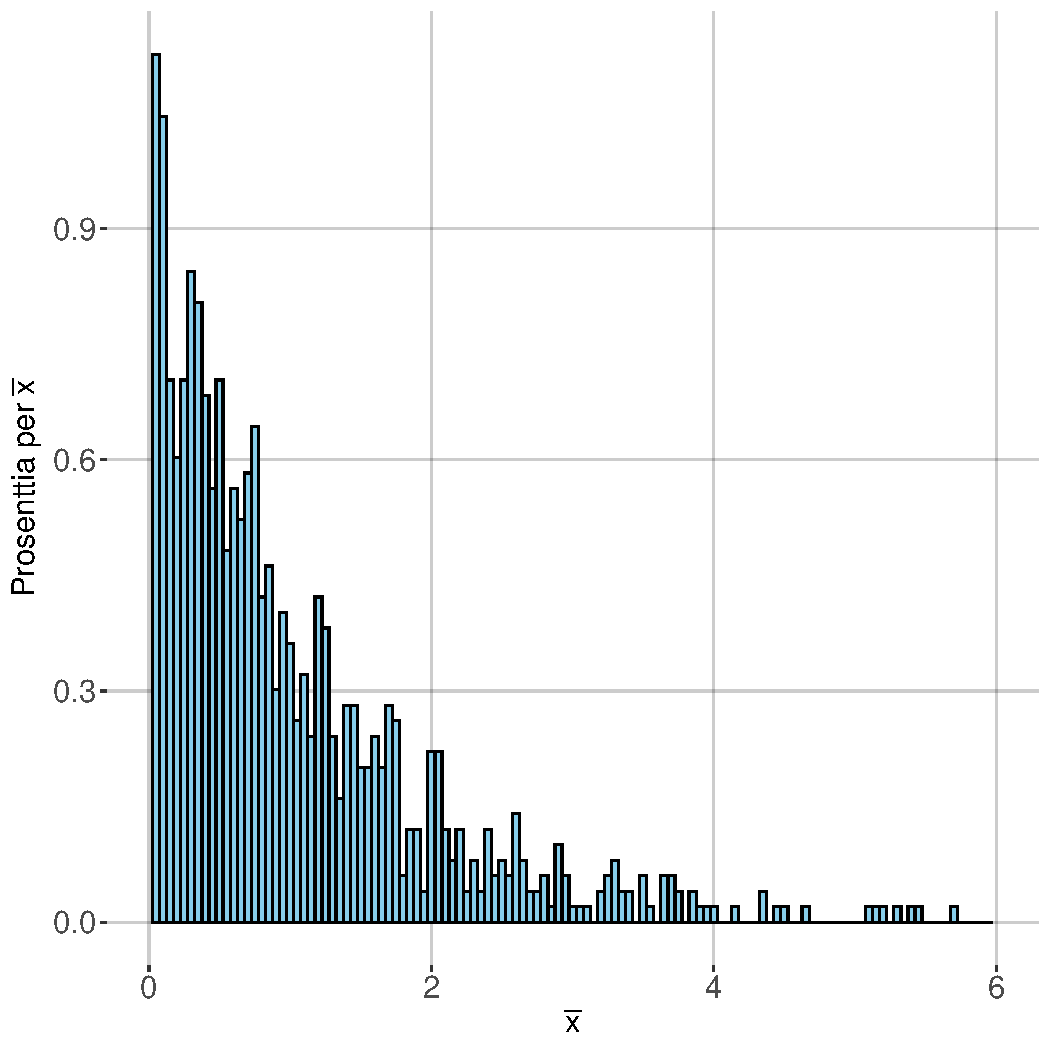
\includegraphics[width=0.7\textwidth, height=0.7\textwidth]{exp-n-1.pdf}
      \caption{Eksponenttijakauma $\mathrm{Exp}\left(1\right)$, $n = 1$ ja $m = 1000$.}
  \end{figure}
\end{center}
\end{frame}

%%%%%%%%%%%%%%%%%%%%%%%%%%%%%%%%%%%

\begin{frame}
  \begin{center}
    \begin{figure}
      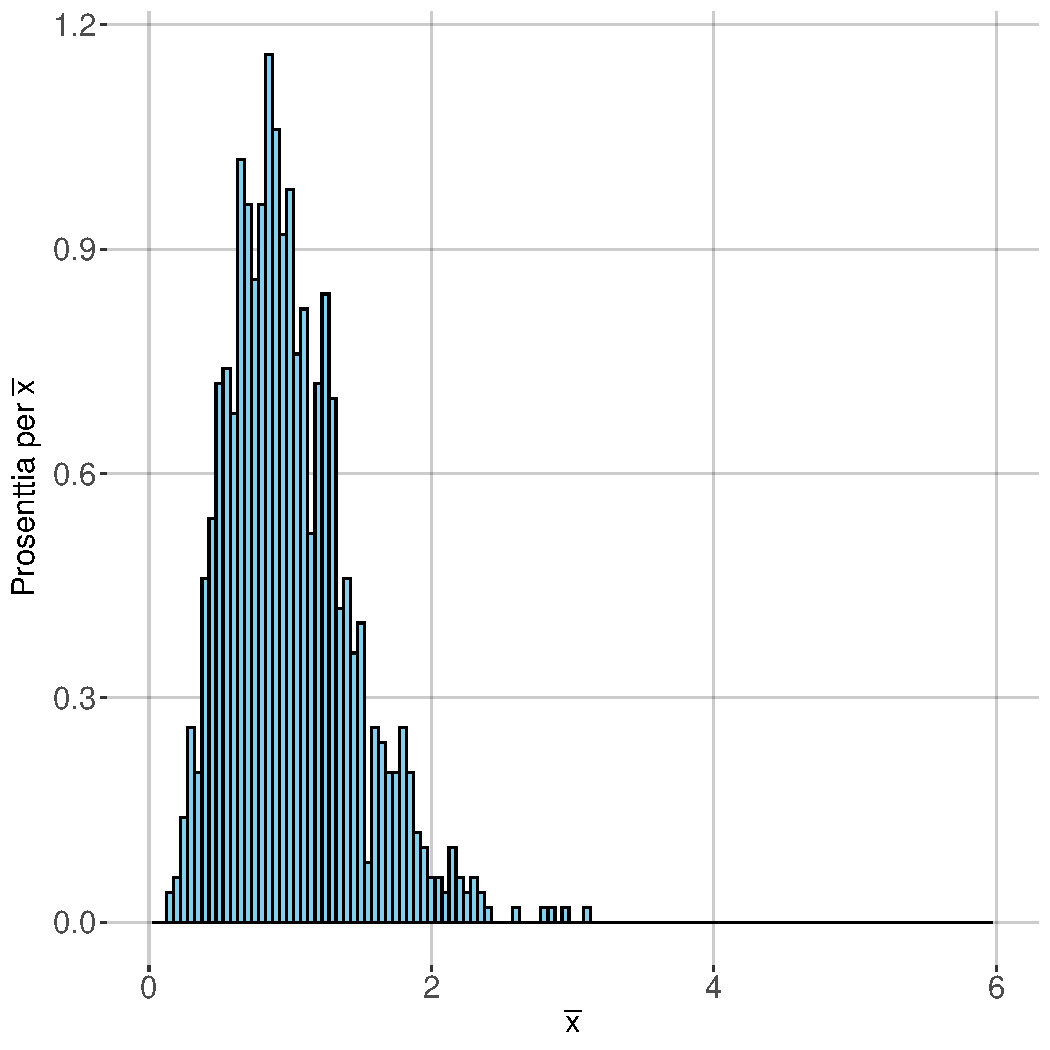
\includegraphics[width=0.7\textwidth, height=0.7\textwidth]{exp-n-5.pdf}
      \caption{Eksponenttijakauma $\mathrm{Exp}\left(1\right)$, $n = 5$ ja $m = 1000$.}
  \end{figure}
\end{center}
\end{frame}

%%%%%%%%%%%%%%%%%%%%%%%%%%%%%%%%%%%

\begin{frame}
  \begin{center}
    \begin{figure}
      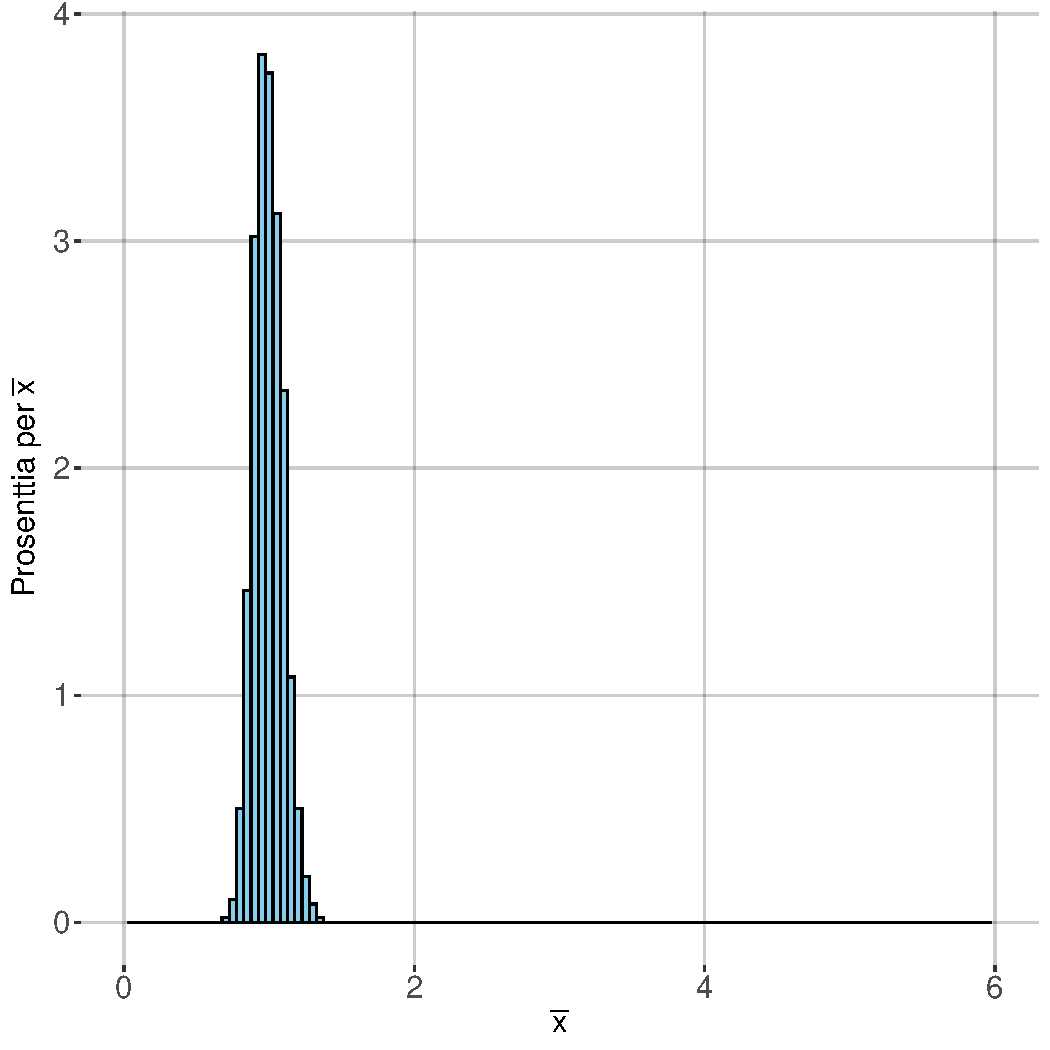
\includegraphics[width=0.7\textwidth, height=0.7\textwidth]{exp-n-100.pdf}
      \caption{Eksponenttijakauma $\mathrm{Exp}\left(1\right)$, $n = 100$ ja $m = 1000$.}
  \end{figure}
\end{center}
\end{frame}

%%%%%%%%%%%%%%%%%%%%%%%%%%%%%%%%%%%

\begin{frame}{Opetustavoite}
  Luennon jälkeen osaamme
  \begin{enumerate}
    \item Kuvata keskeisen raja-arvolauseen intuitiivisesti ja
    \pause
    \item muodostaa likiarvoisen luottamusvälin odotusarvolle perustuen
    keskeiseen raja-arvolauseeseen.
  \end{enumerate}
\end{frame}

%%%%%%%%%%%%%%%%%%%%%%%%%%%%%%%%%%%

\section{Keskeinen raja-arvolause}

%%%%%%%%%%%%%%%%%%%%%%%%%%%%%%%%%%%

\begin{frame}
  \begin{teoreema}
    Olkoon $X_1, X_2, \ldots, X_n$ riippumattomia ja samoin jakautuneita
    satunnaismuuttujia niin, että $0 < \var\left(X_1\right) < \infty$.
    Merkitsemme $\bar X = \frac{1}{n}\sum_{i = 1}^n X_i$, $\mu =
    \mathbb{E}\left(X_1\right)$ ja $\sigma = \sqrt{\var\left(X_1\right)}$.
    Tällöin, kun otoskoko $n$ on suuri, niin
    \begin{equation*}
      \tilde X = \sqrt{n}\frac{\bar X - \mu}{\sigma}
    \end{equation*}
    noudattaa likimain standardinormaalijakaumaa $\n\left(0, 1\right)$,
    \pause
    \begin{equation*}
      \mathbb{P}\left(\tilde X \leq x\right) \approx
      \int_{-\infty}^x \frac{1}{\sqrt{2\pi}}e^{-t^2/2}\,\mathrm{d}t =:
      \Phi\left(x\right).
    \end{equation*}
  \end{teoreema}
\end{frame}

%%%%%%%%%%%%%%%%%%%%%%%%%%%%%%%%%%%

\begin{frame}{\textcolor{magenta}{Intuitio}}
  Kun otoskoko $n$ on suuri, niin melkeinpä $\bar X \sim \n\left(\mu,
  \frac{\sigma^2}{n}\right)$.
  \begin{itemize}
    \item[]
  \end{itemize}
  \pause
  Huom! Dian väite ei pidä täysin paikkaansa vaan antaa vain intuition aiemmille
  simulaatioille.
\end{frame}

%%%%%%%%%%%%%%%%%%%%%%%%%%%%%%%%%%%

\section{Sovellus: likiarvoinen luottamusväli odotusarvolle}

%%%%%%%%%%%%%%%%%%%%%%%%%%%%%%%%%%%

\begin{frame}{Luottamusvälin approksimointi (1)}
  Oletetaan, että satunnaismuuttujan $X$ varianssi $0 < \sigma^2 < \infty$ on
  tiedossa. Tällöin keskeisen raja-arvolauseen mukaan
  \begin{equation*}
    \mathbb{P}\left(z^{(\ell)} \leq \sqrt{n}\frac{\mu - \bar X}{\sigma}
    \leq z^{(u)}\right) \approx 1 - \alpha,
  \end{equation*}
  \pause
  jossa väli $[z^{(\ell)}, z^{(u)}]$ valitaan niin, että
  \begin{equation*}
    \Phi(z^{(u)}) - \Phi(z^{(\ell)}) = 1-\alpha.
  \end{equation*}
  Yllä $F$ on jakauman $\n\left(0,1\right)$ kertymäfunktio.
\end{frame}

%%%%%%%%%%%%%%%%%%%%%%%%%%%%%%%%%%%

\begin{frame}{\textcolor{yellow}{Luottamusvälin approksimointi (2)}}
  Olkoon $z_{1-\alpha/2}$ standardinormaalijakauman $(1-\alpha/2)$-kvantiili.
  Valitsemalla esimerkiksi $z^{(u)} = z_{1 - \alpha/2}$ ja $z^{(\ell)} = -z_{1 -
  \alpha/2}$ päädymme seuraavaan luottamusväliin
  \begin{equation*}
    \left[\bar X - \frac{\sigma z_{1 - \alpha/2}}{\sqrt{n}},
    \bar X + \frac{\sigma z_{1 - \alpha/2}}{\sqrt{n}}\right].
  \end{equation*}
  \pause
  Käytännössä yleensä (tuntematon) keskihajonta korvataan vielä
  otoskeskihajonnalla $\hat\sigma$, sillä suurten lukujen lain perusteella
  $\hat\sigma\approx\sigma$. Päädymme luottamusväliin
  \begin{equation*}
    \left[\bar X - \frac{\hat\sigma z_{1 - \alpha/2}}{\sqrt{n}},
    \bar X + \frac{\hat\sigma z_{1 - \alpha/2}}{\sqrt{n}}\right].
  \end{equation*}
\end{frame}

%%%%%%%%%%%%%%%%%%%%%%%%%%%%%%%%%%%

\begin{frame}{Esimerkki: luottokorttipetokset}
  \begin{itemize}
    \item Otos sisältää luottokorttitapahtumia syyskuulta 2013. Tapahtumia
    kirjattiin kahdelta päivältä
    (Lähde: \href{https://www.kaggle.com/datasets/mlg-ulb/creditcardfraud?resource=download}{\textcolor{red}{Kaggle}}).
    \pause
    \item Luottokorttitapahtumia on yhteensä 284 807, joista 492 luokiteltiin
    petoksiksi.
    \pause
    \item Tavoite: Estimoidaan 95\% luottamusväli petoksien osuudelle
    luottokorttitapahtumista.
  \end{itemize}
\end{frame}

%%%%%%%%%%%%%%%%%%%%%%%%%%%%%%%%%%%

\begin{frame}{Malli}
  \begin{itemize}
    \item Satunnaismuuttuja $X$ noudattaa Bernoullijakaumaa tuntemattomalla
    parametrilla $p$, jossa $p$ on petoksen todennäköisyys.
    \item $\mathbb{P}\left(X = 1\right) = p$ ja $\mathbb{P}\left(X = 0\right) =
    1 - p$, jossa tapahtuma $\{X = 1\}$ indikoi petosta ja $\{X = 0\}$ vastaa
    normaalia luottokorttitapahtumaa.
    \item Havainnot $x_1, \ldots x_{284807}$ ovat binäärisiä (0 tai 1).
    Oletamme, että havainnot ovat riippumattomia ja samoin jakautuneita.
  \end{itemize}
\end{frame}

%%%%%%%%%%%%%%%%%%%%%%%%%%%%%%%%%%%

\begin{frame}{Ratkaisu}
  \begin{itemize}
    \item Voimme laskea $\mathbb{E}\left(X\right) = p$ ja $\var\left(X\right) =
    p(1-p)$.
    \item Suurten lukujen lain mukaan $p \approx \hat p =
    \frac{1}{n}\sum_{i=1}^{284807} x_i$.
    \item Joten voimme approksimoida $95\%$ luottamusvälin seuraavasti
    \begin{equation*}
      \left[\hat p - z_{1 - \alpha/2}\sqrt{\frac{\hat p(1-\hat p)}{n}},
      \hat p + z_{1 - \alpha/2}\sqrt{\frac{\hat p(1-\hat p)}{n}}\right].
    \end{equation*}
  \end{itemize}
\end{frame}

%%%%%%%%%%%%%%%%%%%%%%%%%%%%%%%%%%%

\begin{frame}{Ratkaisu (2)}
  Sijoittamalla lukuarvot
  \begin{itemize}
    \item $\hat p\approx 0.0017$, (\textsf{R} komento \texttt{mean(data)}) ja
    \item $z_{1 - \alpha / 2} \approx 1.96$ (\textsf{R} komento \texttt{qnorm(1
    - 0.05 / 2)})
  \end{itemize}
  saamme luottamusväliksi
  \begin{equation*}
    \approx \left[0.0016, 0.0019\right].
  \end{equation*}
  \pause
  \begin{itemize}
    \item[]
  \end{itemize}
  Luottamusvälin laskemiseen liittyvät yksityiskohdat löytyvät skriptistä
  \texttt{credit.R}. 
\end{frame}

\begin{frame}{Tiivistelmä}
  \begin{enumerate}
    \item Muodostimme intutiivisen käsityksen keskeisestä raja-arvolauseesta
    \begin{itemize}
      \item simulaatioiden ja heurististen laskujen avulla.
    \end{itemize}
    \pause
    \item Sovelsimme keskeistä raja-arvolausetta luottokorttipetoksiin
    \begin{itemize}
      \item laskemalla likiarvoistettuja luottamusvälejä petoksen
      todennäköisyydelle.
    \end{itemize}
  \end{enumerate}
  \begin{itemize}
    \item[]
  \end{itemize}
  \pause
  Kaikki materiaalit löytyvät osoitteesta
  \url{https://github.com/perej1/clt-teaching}.
\end{frame}
\end{document}
